% Created 2024-10-02 Wed 19:12
% Intended LaTeX compiler: pdflatex
\documentclass[11pt]{article}
\usepackage[utf8]{inputenc}
\usepackage[T1]{fontenc}
\usepackage{graphicx}
\usepackage{longtable}
\usepackage{wrapfig}
\usepackage{rotating}
\usepackage[normalem]{ulem}
\usepackage{amsmath}
\usepackage{amssymb}
\usepackage{capt-of}
\usepackage{hyperref}
\usepackage{minted}
\usepackage[a4paper, margin=2.5cm]{geometry}
\usepackage{minted}
\usepackage{fontspec}
\setmonofont{Iosevka}
\setminted{fontsize=\small, frame=single, breaklines=true}
\usemintedstyle{emacs}
\usepackage[backend=biber,style=apa]{biblatex}
\addbibresource{citation.bib}
\usepackage{float}
\author{Baley Eccles - 652137 and Tyler Robards - 651790}
\date{\textit{{[}2024-09-20 Fri 18:34]}}
\title{ENG204 - Signals and Linear Systems - Assignment 1.4}
\hypersetup{
 pdfauthor={Baley Eccles - 652137 and Tyler Robards - 651790},
 pdftitle={ENG204 - Signals and Linear Systems - Assignment 1.4},
 pdfkeywords={},
 pdfsubject={},
 pdfcreator={Emacs 29.4 (Org mode 9.8)}, 
 pdflang={English}}
\begin{document}

\maketitle
\tableofcontents

\section{Laplace Transforms to solve Partial Differential Equations}
\label{sec:org10fdf15}
\subsection{a}
\label{sec:orga8c94fb}
\begin{align*}
\frac{d^3y}{d^3t}+5\frac{d^2y}{d^2t}+9\frac{dy}{dt}+45y &= -t^2u(t)+2e^{-t}u(t-2) \\
\leftrightarrow^{\mathcal{L}} s^3Y(s)+5s^2Y(s)+9sY(s)+45Y(s) &= -\frac{2}{s^{3}} +2e^{-2s}\frac{1}{s+1} \\
Y(s) = \frac{-\frac{2}{s^{3}} +2\frac{e^{-2s}}{s+1}}{s^3+5s^2+9s+45}&\\
\textrm{Partial Fractions From WolframAlpha}& \\
Y(s)=\frac{2e^{-2s}}{(s+1)(s+5)(s^2+9)}-&\frac{2}{s^3(s+5)(s^2+9)} \\
\textrm{From WolframAlpha}& \\
y(t)=(675 u(t - 2) (-15 e^{10 - 5 t} + 51 e^{2 - t} + &8 \sin(6 - 3 t) - 36 \cos(6 - 3 t)) \\
 + 4 (-3825 t^2 + 1530 t + 81 e^{-5 t} - 375 \sin(3 t)& - 625 \cos(3 t) + 544))/688500
\end{align*}
\subsection{b}
\label{sec:org178c534}
\subsubsection{1}
\label{sec:org11c2bad}
\begin{align*}
\mathcal{L}\left\{\frac{\partial f}{\partial x}\right\}+\mathcal{L}\left\{\frac{\partial f}{\partial t}\right\}+\mathcal{L}\left\{f\right\}&=0\\
\frac{\partial F}{\partial x}+sF(x,s)-f(x,0)+F(x,s)&=0\\
\textrm{Inital condition }f(x,0)&=sin(x):\\
\frac{\partial F}{\partial x}+(s+1)F(x,s)&=sin(x)
\end{align*}
\subsubsection{2}
\label{sec:org7f79dec}
Using the integrating factor technique
\begin{align*}
\mu(x)&=e^{\int(s+1)dx}=e^{(s+1)x} \\
\Rightarrow &e^{(s + 1)x} \frac{\partial F}{\partial x} + (s + 1)e^{(s + 1)x}F = e^{(s + 1)x}\sin(x)\\
\Rightarrow&\frac{\partial}{\partial x}\left(e^{(s + 1)x}F\right) = e^{(s + 1)x}\sin(x)\\
\Rightarrow & e^{(s + 1)x}F = \int e^{(s + 1)x}\sin(x) dx + C(s) \\
&\textrm{From Calculator}\\
\Rightarrow &e^{(s + 1)x}F = \frac{e^{(s + 1)x}}{(s + 1)^2 + 1}((s + 1)\sin(x) - \cos(x)) + C(s)\\
\Rightarrow & F(x, s) = \frac{(s + 1)\sin(x) - \cos(x)}{(s + 1)^2 + 1} + C(s)e^{-(s + 1)x}
\end{align*}
\subsubsection{3}
\label{sec:org0b21eaa}
\begin{align*}
F(0, s) &= \frac{(s + 1)\sin(0) - \cos(0)}{(s + 1)^2 + 1} + C(s)e^{-(s + 1)0} \\
\Rightarrow C &= \frac{1}{s^2+2s+2} \\
\Rightarrow  F(x, s) &= \frac{(s + 1)\sin(x) - \cos(x)}{(s + 1)^2 + 1} + \frac{e^{-(s + 1)x}}{s^2+2s+2}
\end{align*}
\subsubsection{4}
\label{sec:org8942e19}
\begin{align*}
\mathcal{L}\left\{F(x, s)\right\} &= \mathcal{L}\left\{\frac{(s + 1)\sin(x) - \cos(x)}{(s + 1)^2 + 1} + \frac{e^{-(s + 1)x}}{s^2+2s+2}\right\} \\
f(x,t)&=e^{-t}[\sin(x-t)+\sin(t-x)u(t-x)]
\end{align*}
\subsubsection{5}
\label{sec:orge6fc743}
\begin{align*}
\frac{\partial f}{\partial x}&=e^{-t}\cos(x-t)-\cos(t-x)u(t-x)-\sin(t-x)\delta(t-x)\\
\frac{\partial f}{\partial t}&=-e^{-t}[\sin(x-t)+\sin(t-x)u(t-x) \\
&+e^{-t}[-\cos(x-t)+\cos(t-x)u(t-x)+\sin(t-x)\delta(t-x)] \\
\frac{\partial f}{\partial x}+\frac{\partial f}{\partial t}+f &=e^{-t}\cos(x-t)-\cos(t-x)u(t-x)-\sin(t-x)\delta(t-x)\\
&-e^{-t}[\sin(x-t)+\sin(t-x)u(t-x)]\\
&+e^{-t}[-\cos(x-t)+\cos(t-x)u(t-x)+\sin(t-x)\delta(t-x)]\\
&+e^{-t}[\sin(x-t)+\sin(t-x)u(t-x)]
\end{align*}
Plugging this into a calculator shows that it equals zero, as required.
\begin{minted}[]{octave}
clc
clear
close all
set(0, 'DefaultAxesFontSize', 40);
set(0, 'DefaultTextFontSize', 40);
set(0, 'DefaultLegendFontSize', 40);
x = linspace(0, 10, 100);
t = linspace(0, 10, 100);
[X, T] = meshgrid(x, t);
f = exp(-T) .* (sin(X - T) + sin(T - X) .* (T >= X));

surf(X, T, f);
xlabel('x');
ylabel('t');
zlabel('f(x,t)');
title('Solution of the PDE f(x,t)');
filename = sprintf('ENG204-Assignment-4-Part-b.png');
print(filename, '-dpng', '-r100');
\end{minted}
\begin{FIGURE}
\begin{figure}[H]
\centering
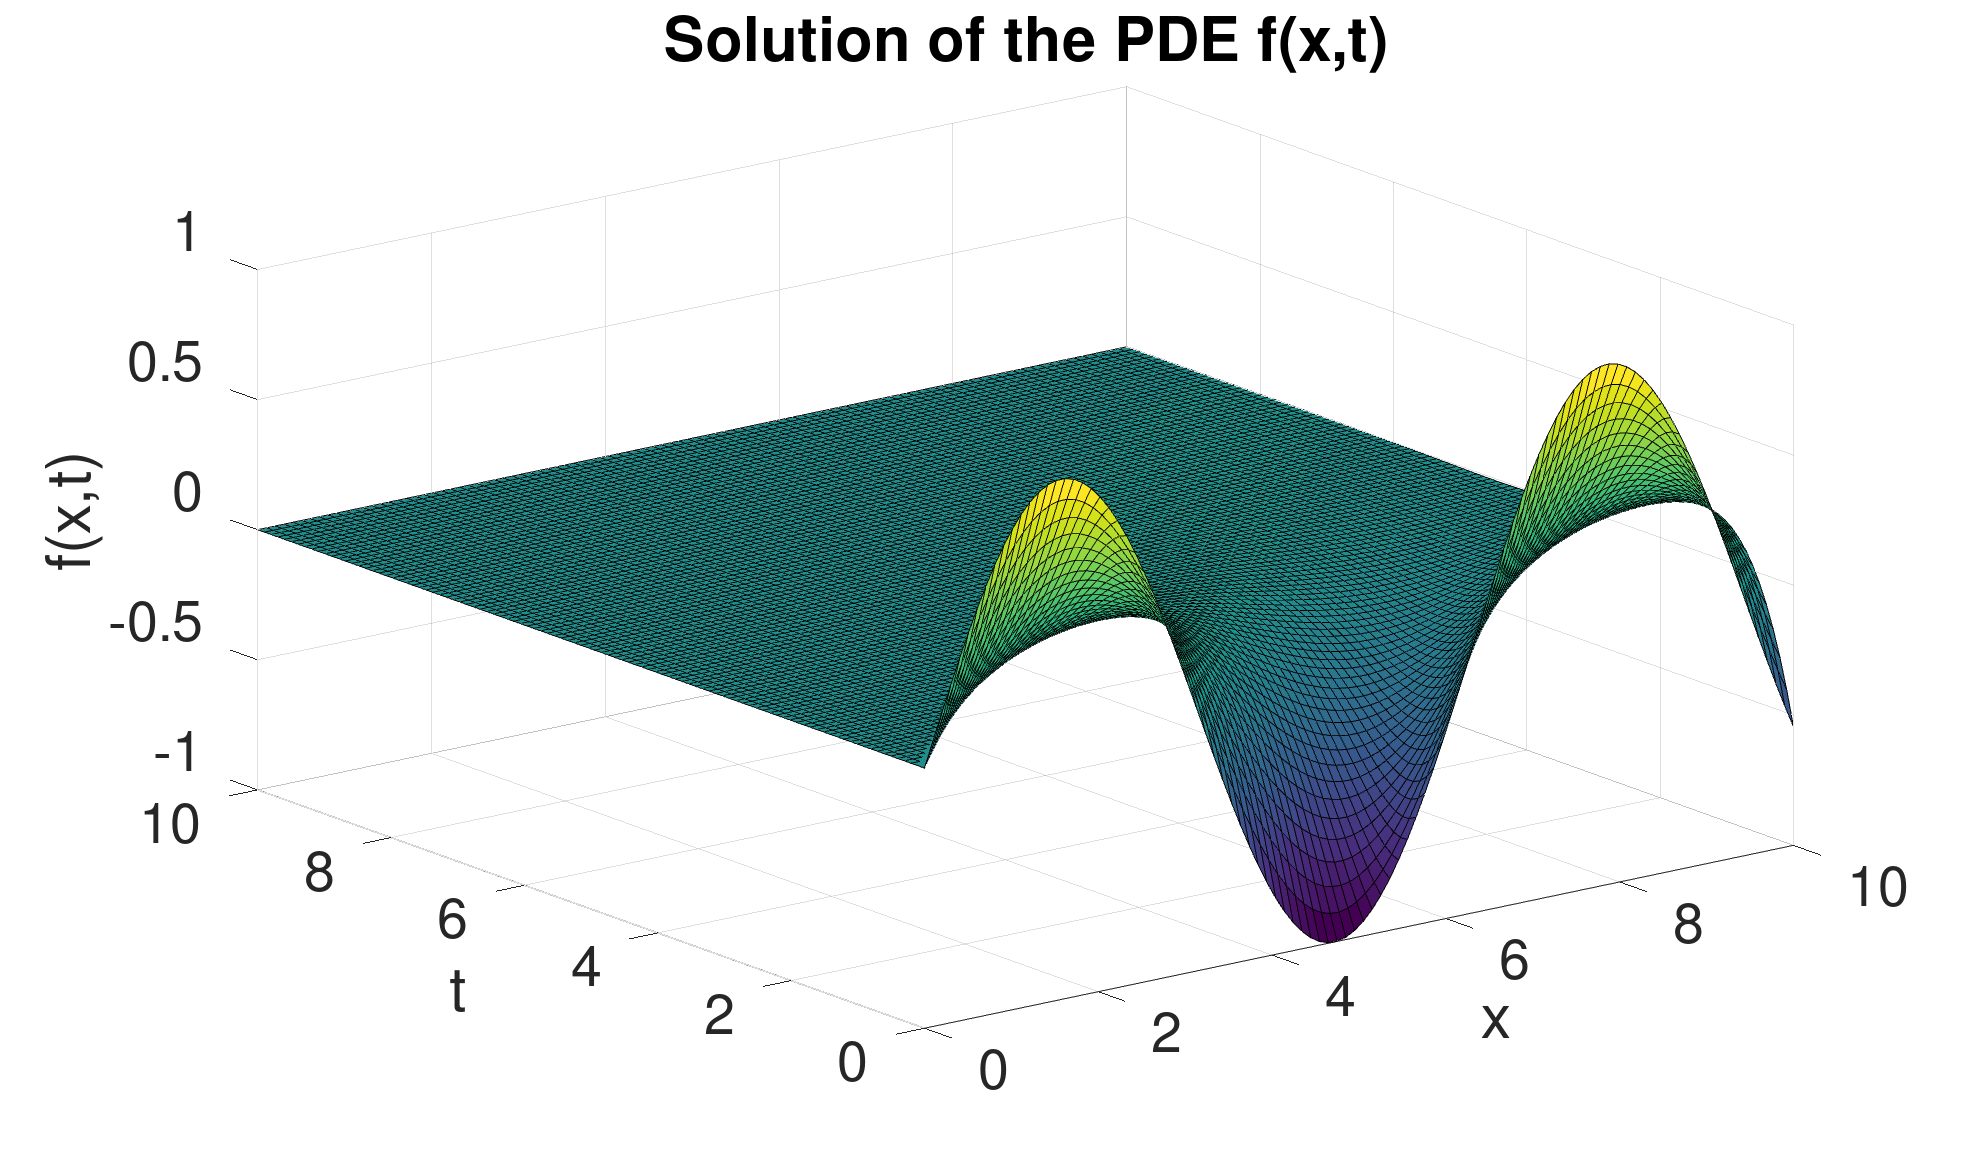
\includegraphics[width=.9\linewidth]{ENG204-Assignment-4-Part-b.png}
\caption{Plot of the solution to the PDE}
\end{figure}
\end{FIGURE}
\subsection{c}
\label{sec:org5e09181}
Take the Laplace transform:
\begin{align*}
\frac{\partial f}{\partial t}&=\alpha \frac{\partial^2f}{\partial x^2} \\
&\updownarrow \mathcal{L}\\
sF(x,s)-f(x,0) &=\alpha \frac{\partial ^2F(x,s)}{\partial x^2} \\
sF(x,s)-T_0\sin(\pi x) &=\alpha \frac{\partial ^2F(x,s)}{\partial x^2} \\
\alpha \frac{\partial ^2F(x,s)}{\partial x^2}-sF(x,s) &= -T_0\sin(\pi x)\\
\end{align*}
Solving the homogeneous part:
\begin{align*}
\alpha \frac{\partial^2F(x,s)}{\partial x^2}-sF(x,s) &= 0 \\
\Rightarrow F(x,s)&=Ae^{\sqrt{\frac{s}{\alpha}}x}+Be^{-\sqrt{\frac{s}{\alpha}}x}
\end{align*}
Solving particular solution:
\begin{align*}
F(x,s) &= C\sin(\pi x) \\
\Rightarrow -\pi^2C\sin(\pi x)-\frac{s}{\alpha}C\sin(\pi x) &= -\frac{T_0}{\alpha}\sin(\pi x)
\Rightarrow C=\frac{T_0}{\pi^2\alpha+s}
\end{align*}
Combining the solutions
\begin{align*}
F(x,s) &= \frac{T_0}{\pi^2\alpha+s}\sin(\pi x) + Ae^{\sqrt{\frac{s}{\alpha}}x}+Be^{-\sqrt{\frac{s}{\alpha}}x} \\
\end{align*}
Boundary conditions:
\begin{align*}
x=0:& \\
F(0,s) &= A+B+\frac{T_0}{\pi^2\alpha+s}\cdot 0 = 0 \\
\textrm{and } x=2:& \\
F(2,s) &= Ae^{2\sqrt{\frac{s}{\alpha}}}+Be^{-2\sqrt{\frac{s}{\alpha}}}+\frac{T_0}{\pi^2\alpha+s}\sin(2\pi) = 0 \\
\Rightarrow A=0 &\textrm{ and } B=0
\end{align*}
Hence:
\begin{align*}
F(x,s) &= \frac{T_0}{\pi^2\alpha+s}\sin(\pi x)\\
\end{align*}
\begin{minted}[]{octave}
clc
clear
close all
set(0, 'DefaultAxesFontSize', 40);
set(0, 'DefaultTextFontSize', 40);
set(0, 'DefaultLegendFontSize', 40);
warning('off','all');

x = 0:0.01:2;
s = 0:0.1:10;

To=1;
a=0.5;

[X, S] = meshgrid(x, s);

FS = (To ./ (a * (pi^2 + (S / a)))) .* sin(pi * X);

figure;
surf(X, S, FS);
xlabel('X-axis');
ylabel('S-axis');
zlabel('F-axis');
title('3D Surface Plot of F(s,x)=(T0/(a*(pi^2+(s/a))))sin(pi*x)');
colorbar;
shading interp;
filename = sprintf('ENG204-Assignment-4-Part-c.png');
print(filename, '-dpng', '-r100');
\end{minted}

\begin{FIGURE}
\begin{figure}[H]
\centering
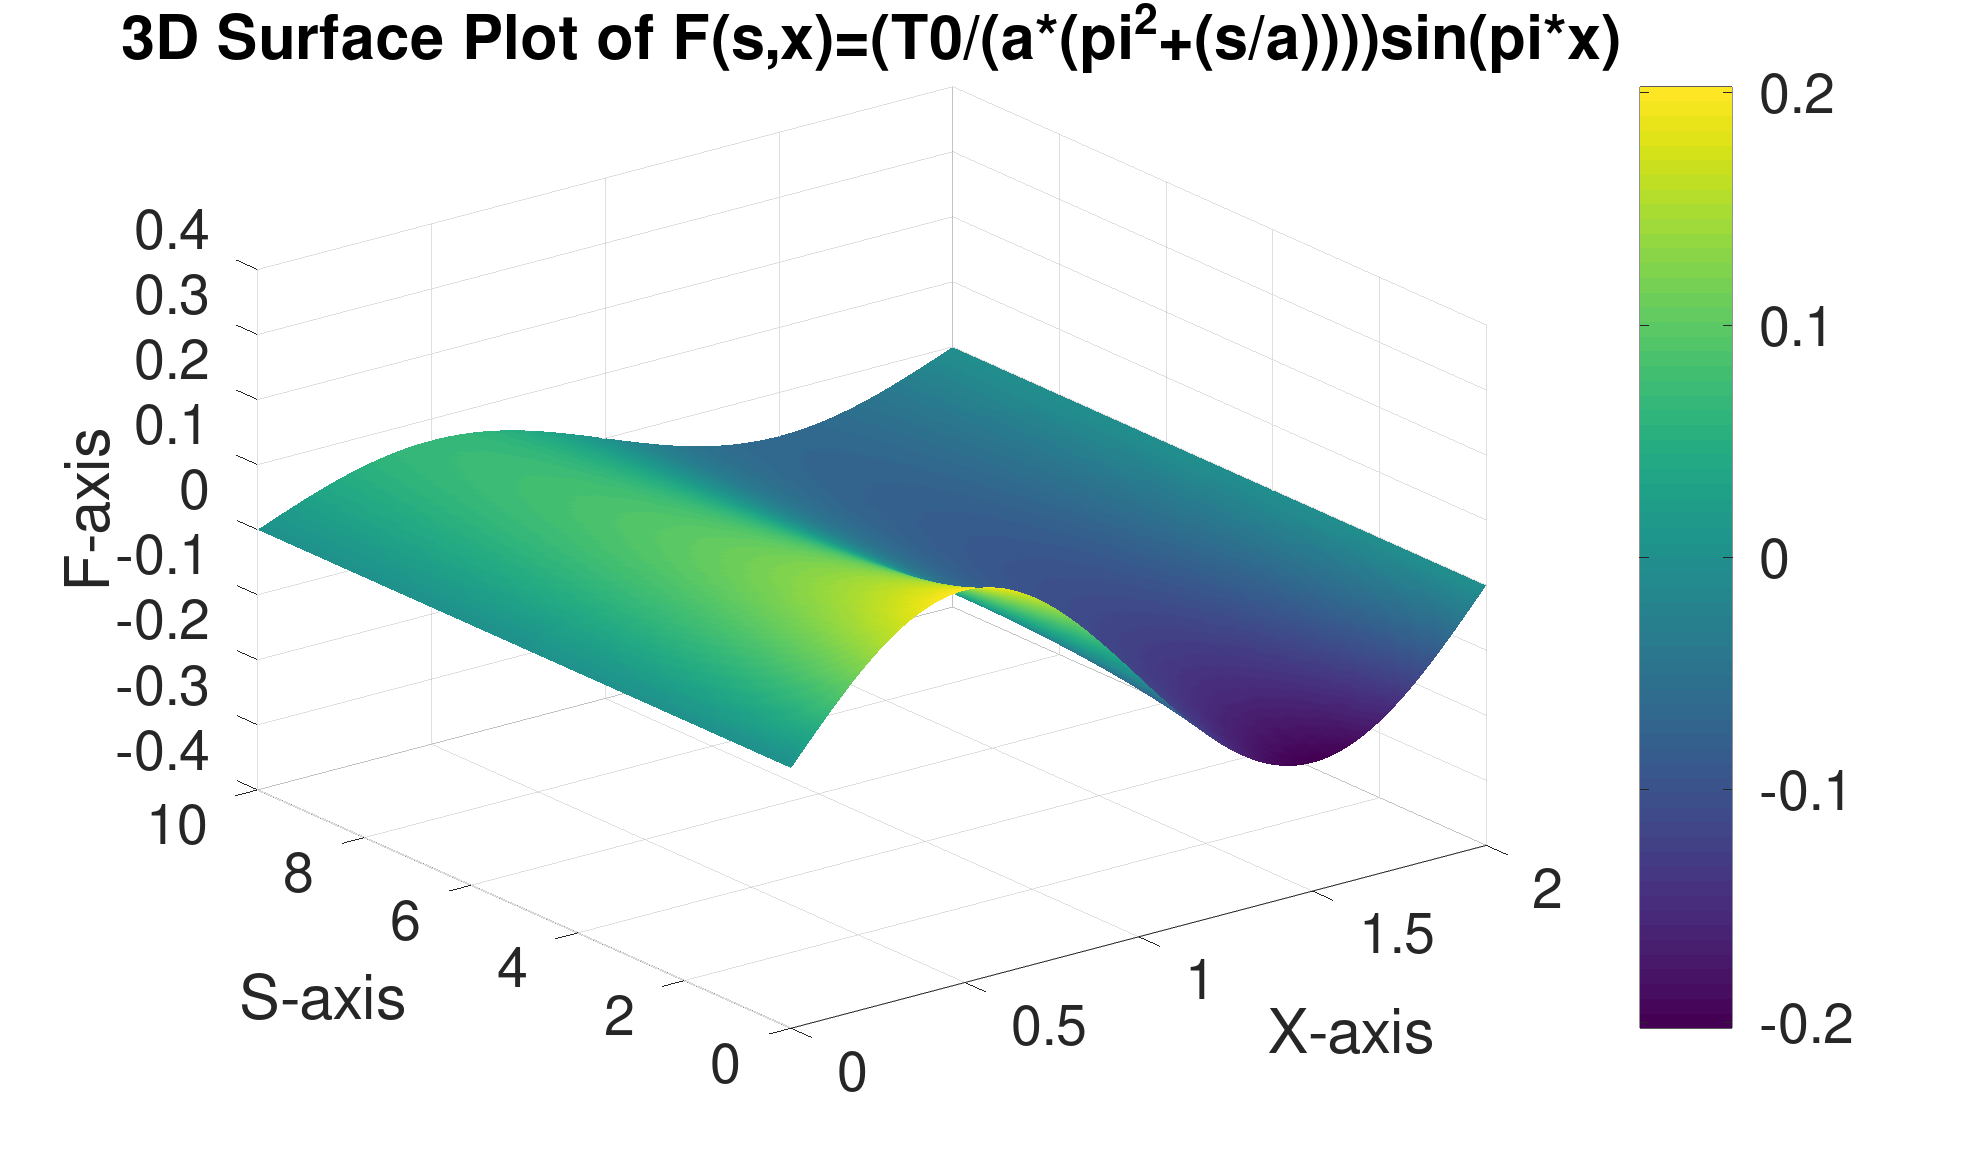
\includegraphics[width=.9\linewidth]{ENG204-Assignment-4-Part-c.png}
\caption{Plot of the solution to the heat equation}
\end{figure}
\end{FIGURE}
\section{Harmonic Filter}
\label{sec:org6411159}
Output of the \texttt{harmonic\_filter.p} with student IDs 652137 and 651790:
\begin{verbatim}
Please use a system voltage of 33 kV
Please use a capacitor of size 6 MVAR
Please use a quality factor of 28
Please use an inductance L2 of 18 mH
Your filter must reject harmonic numbers 3 and 7
\end{verbatim}
These were used to derive find the values for the resistors, inductors and capacitors:
\begin{align*}
C_1&=\frac{6M}{100\pi(33k)^2}&=17\mu F \\
R_1&=28\cdot 18m\cdot 1440 &= 725.6 \\
C_1&=\frac{1}{18m(1440)^2}&=26.8\mu F \\
L_1&=\frac{1}{17.53\mu\cdot 1440^2}&=27.5mH
\end{align*}
Taking the laplace transform of each component
\begin{align*}
ZC_1&=1/(s\cdot C_1) \\
ZR_1&=R_1 \\
ZC_2&=1/(s\cdot C_2) \\
ZL_1&=L_1\cdot s \\
ZL_2&=L_2\cdot s \\
\end{align*}
We can combine these into one impedance:
\begin{align*}
Z_{equ}&=ZL_1+ZC_1+(1/((1/ZL_2)+(1/ZR_)+(1/ZC_2)))
\end{align*}
And using a current divider we can find the transfer function:
\begin{align*}
H(s)=\frac{I_o(s)}{I_h(s)} &= (Z_{equ}/(R_{+Load}+Z_{equ}))
\end{align*}
Which comes out to be:
\begin{align*}
H(s) = \frac{
\begin{array}{c}
    59208000 \pi s^{4} + 3044259360 \pi s^{3} + 122715487600000 \pi s^{2} \\
    + 637762222186155 s^{2} + 19822138465215339 s + 799039470485069302500
    \end{array}}{
    \begin{array}{c}
    59208000 \pi s^{4} + 3044259360 \pi s^{3} + 676118355000 s^{3} \\
    + 122715487600000 \pi s^{2} + 672525761415255 s^{2} + 1421156309677465339 s \\
    + 799039470485069302500
\end{array}}
\end{align*}
Here is the code that was used to calculate the transfer function:
\begin{minted}[]{octave}
clc
clear
close all
warning('off','all');
pkg load symbolic

% Given values
Vsys=33*10^3;
Csize=6*10^6;
Q=28;
L2=18*10^-3;
n1=3;
n2=7;
RLoad=100;

%Frequecnies and w_m
f=50;
f1=f*n1;
f2=f*n2;
fm=sqrt(f1*f2);
wm=2*pi*fm;

% Calculate Capacitors, resistor and inductor
C1=(Csize)/(100*pi*Vsys^2);
R1=Q*L2*wm;
C2=1/(L2*wm^2);
L1=1/(C1*wm^2);

%% Equivelant impeadance using laplace transform
syms s
ZC1=1/(s*C1);
ZR1=R1;
ZC2=1/(s*C2);
ZL1=L1*s;
ZL2=L2*s;
Zequ=ZL1+ZC1+(1/((1/ZL2)+(1/ZR1)+(1/ZC2)));

% Transfer function using current divider
TransferFunction = (Zequ/(RLoad+Zequ));
TransferFunction=factor(TransferFunction);

[den,num]=numden(TransferFunction);
zeros=vpasolve(num(2)==0,s)
poles=vpasolve(den(1)==0,s)

\end{minted}
Here is the code that uses the transfer function:
\begin{minted}[]{octave}
clc
clear
close all
pkg load control

set(0, 'DefaultAxesFontSize', 40);
set(0, 'DefaultTextFontSize', 40);
set(0, 'DefaultLegendFontSize', 40);



poles=[-2306.1292101125216811843091219593, -898.74275697138288696284712221959, -240.72250145498954243549730861195 - 1419.3905739866029604915898580966*i, -240.72250145498954243549730861195 + 1419.3905739866029604915898580966*i];
zeros=[- 17.672679232183922726973141504934 - 2134.9568788579925354983418033515*i, - 17.672679232183922726973141504934 + 2134.9568788579925354983418033515*i, - 8.0355102995882391545947238890328 + 970.73385217099055769742907468453*i, - 8.0355102995882391545947238890328 - 970.73385217099055769742907468453*i];
gain = 1;

sys = tf(poly(zeros), poly(poles));
% 1. Calculate the impulse response
figure;
impulse(sys);
title('Impulse Response of the System');
grid on;
filename = sprintf('ENG204-Assignment-4-Impulse.png');
print(filename,'-dpng','-r100');

% 2. Calculate the step response
figure;
step(sys);
title('Step Response of the System');
grid on;
filename = sprintf('ENG204-Assignment-4-Step.png');
print(filename,'-dpng','-r100');

%% 3. Produce Bode plots
% Magnitude and phase
figure;
bode(sys);
title('Bode Plot of the System');
grid on;
filename = sprintf('ENG204-Assignment-4-Bode1.png');
print(filename,'-dpng','-r100');

% Magnitude in HZ
w = logspace(-2, 6, 1000);
[mag, ~, wout] = bode(sys, w);
mag_dB = 20*log10(squeeze(mag));
fout = wout / (2 * pi);
figure;
semilogx(fout, mag_dB);
grid on;
title('Magnitude Response of the Transfer Function');
xlabel('Frequency (Hz)');
ylabel('Magnitude (dB)');

filename = sprintf('ENG204-Assignment-4-Bode2.png');
print(filename,'-dpng','-r100');
% 4. Calculate the output current for a pure 50 Hz sinusoid
t = 0:0.001:1;
input_current_50Hz =sin(2 * pi * 50 * t);
output_current_50Hz = lsim(sys, input_current_50Hz, t);
figure;
plot(t, output_current_50Hz);
title('Output Current for 50 Hz Sinusoid Input');
xlabel('Time (s)');
ylabel('Output Current i_io(t)');
grid on;
filename = sprintf('ENG204-Assignment-4-50Hz.png');
print(filename,'-dpng','-r100');

% 5. Calculate the output current for 350Hz
input_current_350Hz = sin(2 * pi * 350 * t);
output_current_350Hz = lsim(sys, input_current_350Hz, t);
figure;
plot(t, output_current_350Hz);
title('Output Current for 350 Hz Sinusoid Input');
xlabel('Time (s)');
ylabel('Output Current i_io(t)');
grid on;
filename = sprintf('ENG204-Assignment-4-350Hz.png');
print(filename,'-dpng','-r100');

% 6. Calculate the output current for a superposition of fundamental and harmonic currents
t = 0:0.0001:0.1;
input_current_superposition = sin(2 * pi * 50 * t) + sin(2 * pi * 150 * t) + sin(2 * pi * 350 * t);
output_current_superposition = lsim(sys, input_current_superposition, t);
filtered_output_current = lsim(sys, output_current_superposition, t);
figure;
hold on;
plot(t, output_current_superposition, 'b', 'DisplayName', 'Unfiltered Output Current');
plot(t, filtered_output_current, 'r', 'DisplayName', 'Filtered Output Current');
hold off;
title('Output Current for Superposition of Fundamental and Harmonics');
xlabel('Time (s)');
ylabel('Output Current i_io(t)');
grid on;
legend show;
filename = sprintf('ENG204-Assignment-4-Super.png');
print(filename, '-dpng', '-r100');
\end{minted}
\begin{FIGURE}
\begin{figure}[H]
\centering
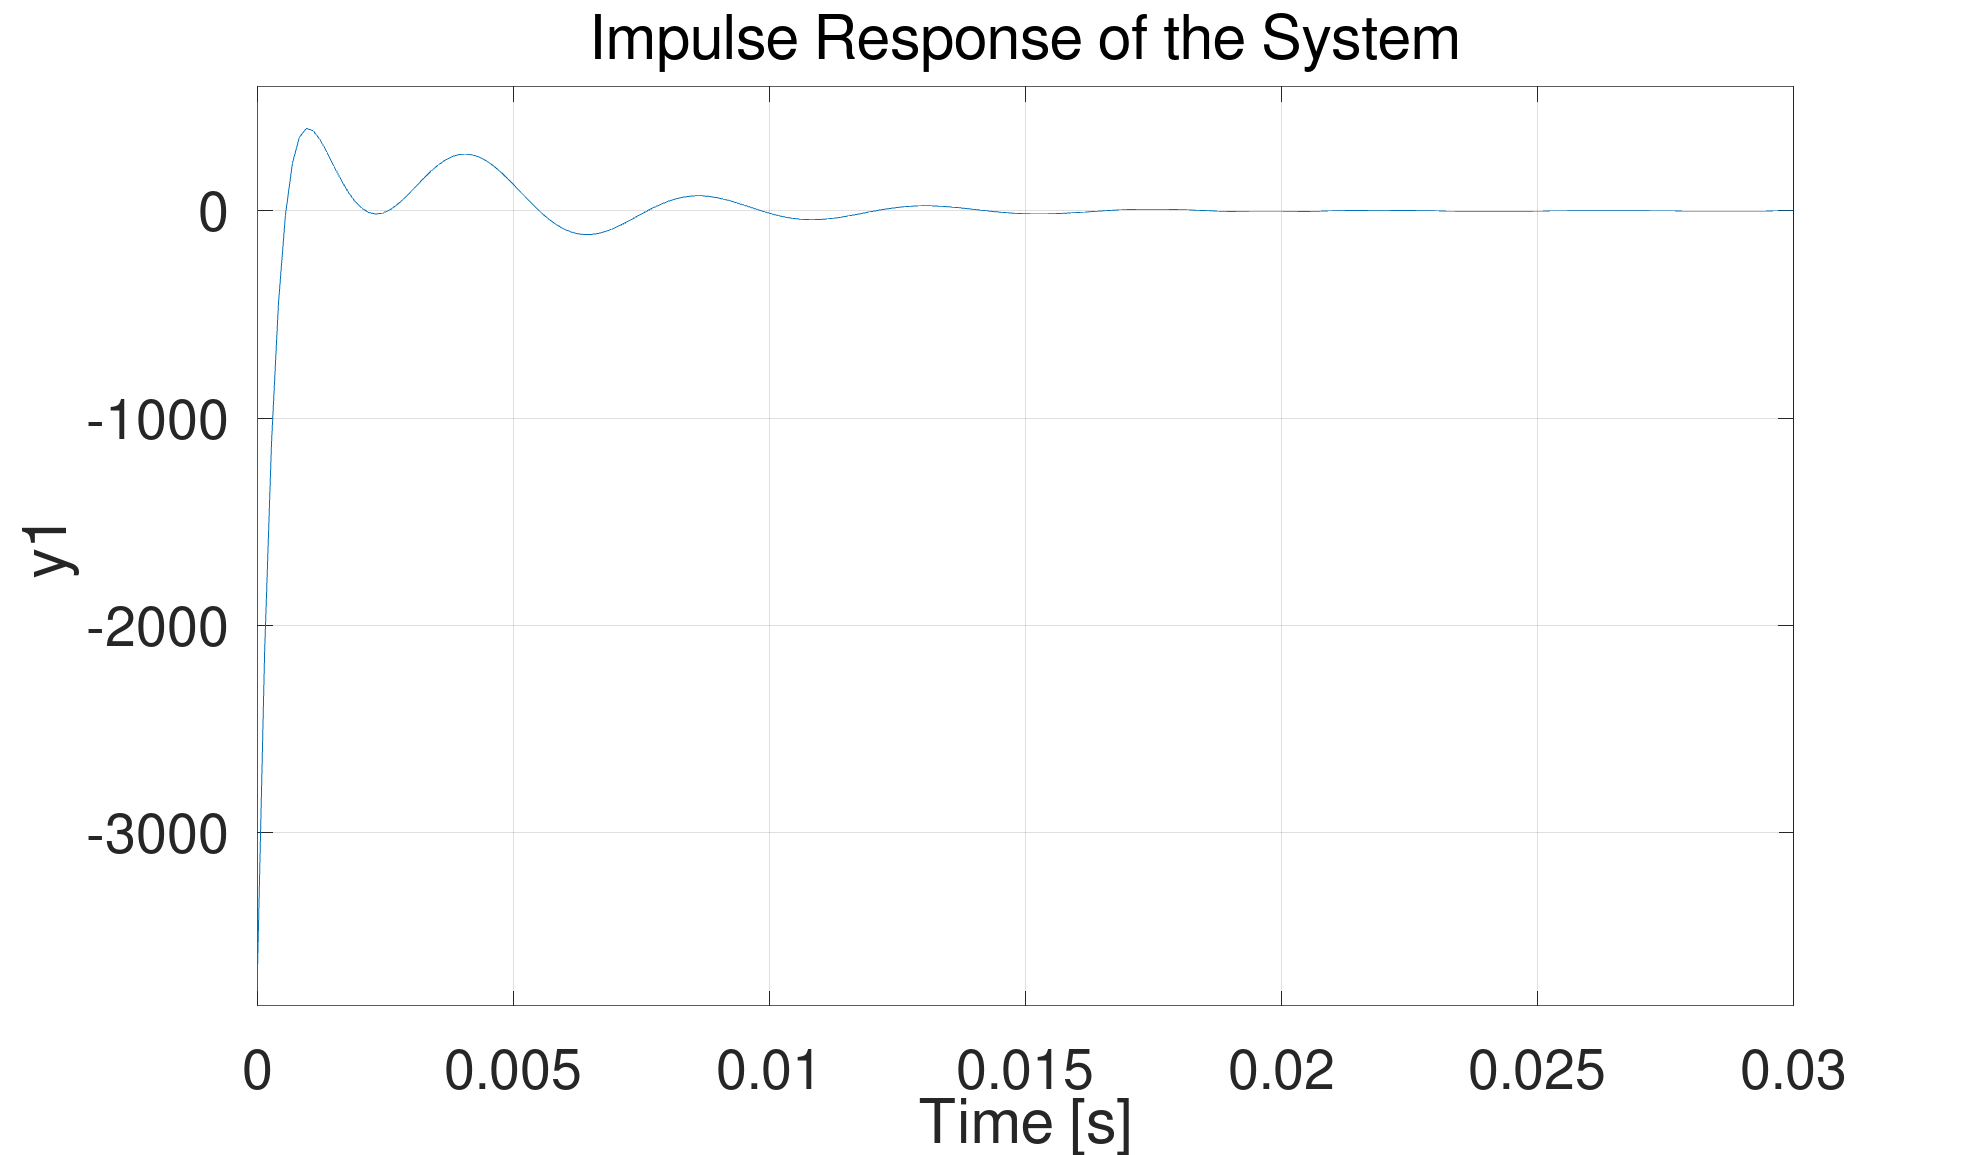
\includegraphics[width=.9\linewidth]{ENG204-Assignment-4-Impulse.png}
\caption{Impulse response of the transfer function.}
\end{figure}
\end{FIGURE}
\begin{FIGURE}
\begin{figure}[H]
\centering
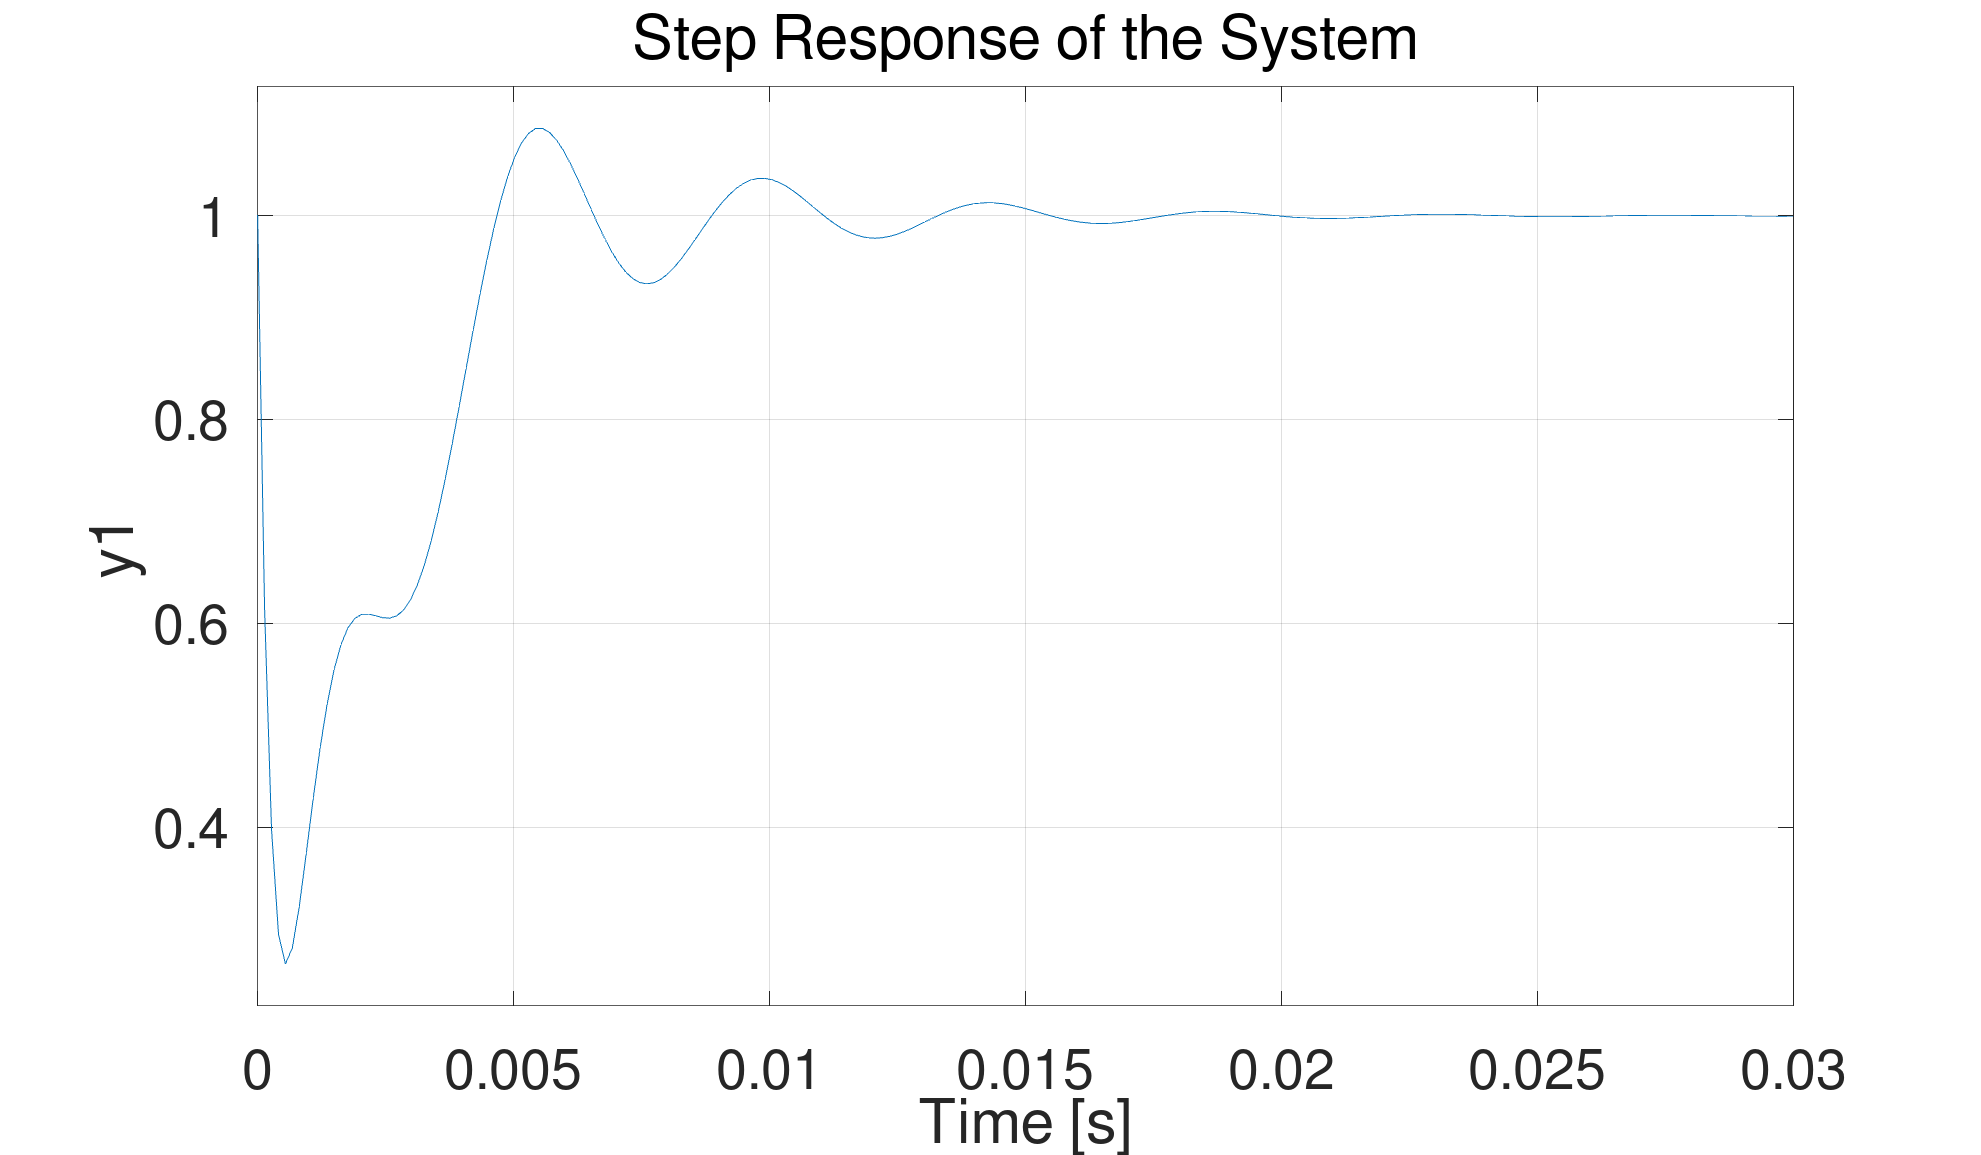
\includegraphics[width=.9\linewidth]{ENG204-Assignment-4-Step.png}
\caption{Step response of the transfer function.}
\end{figure}
\end{FIGURE}
\begin{FIGURE}
\begin{figure}[H]
\centering
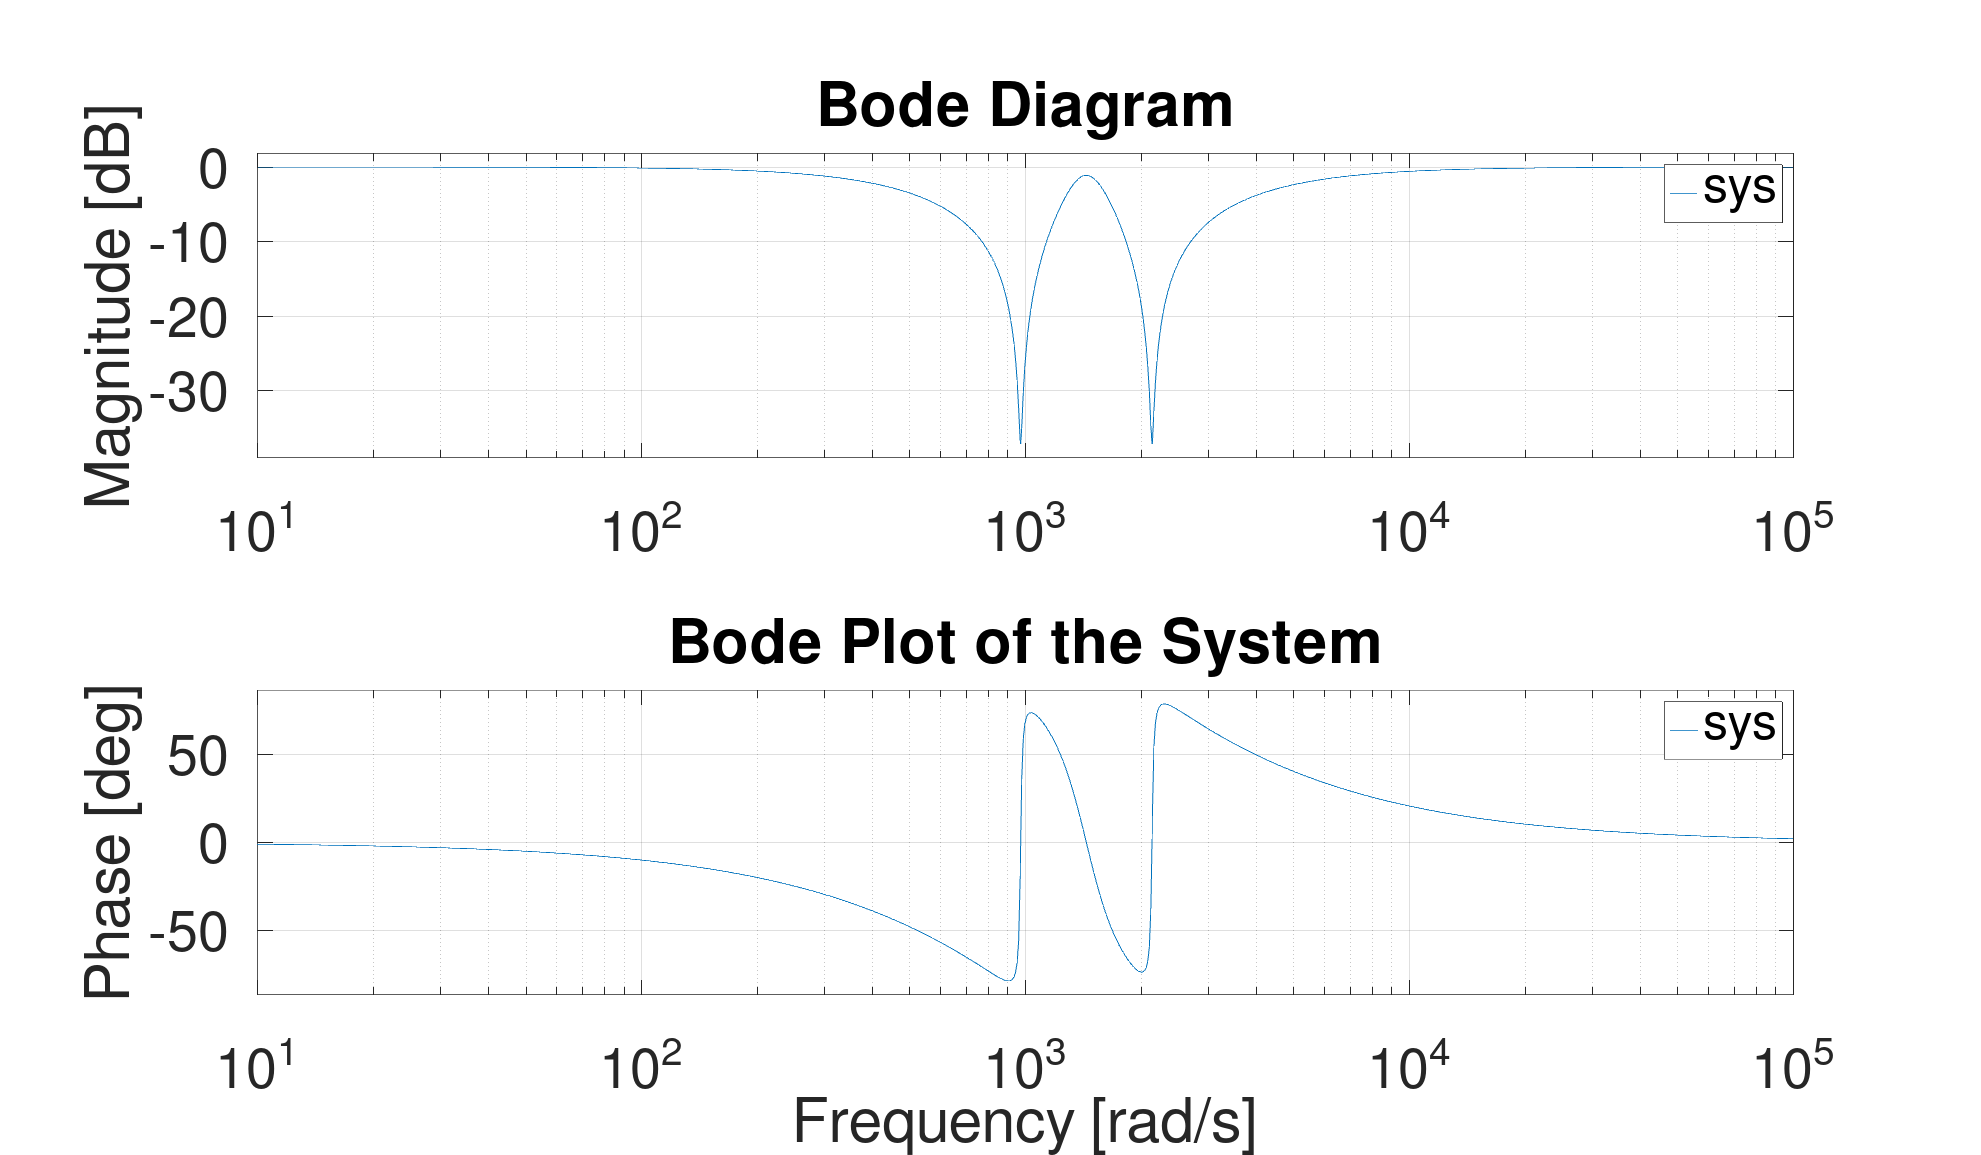
\includegraphics[width=.9\linewidth]{ENG204-Assignment-4-Bode1.png}
\caption{Bode magnitude and phase of the transfer function.}
\end{figure}
\end{FIGURE}
\begin{FIGURE}
\begin{figure}[H]
\centering
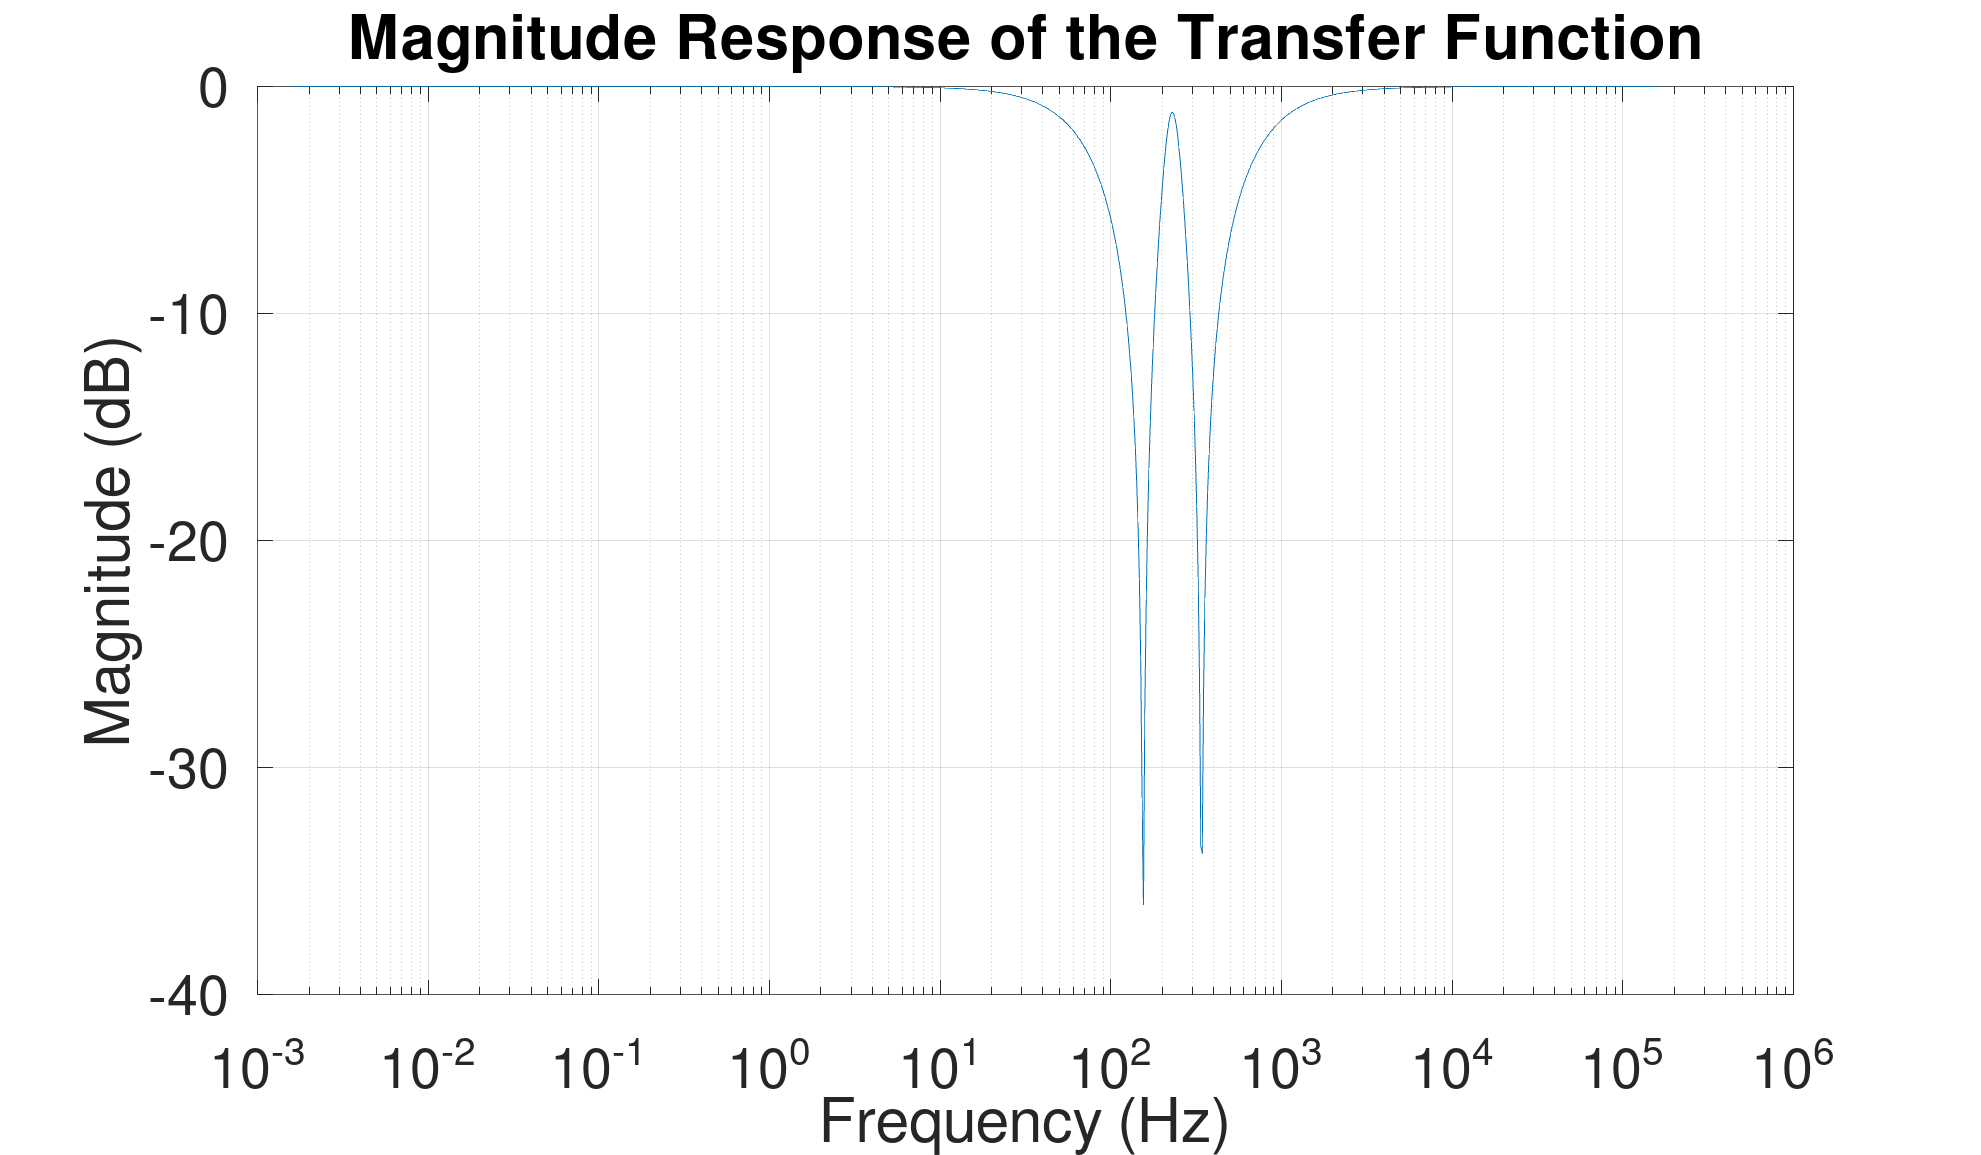
\includegraphics[width=.9\linewidth]{ENG204-Assignment-4-Bode2.png}
\caption{Bode magnitude of the transfer function in Hertz.}
\end{figure}
\end{FIGURE}
\begin{FIGURE}
\begin{figure}[H]
\centering
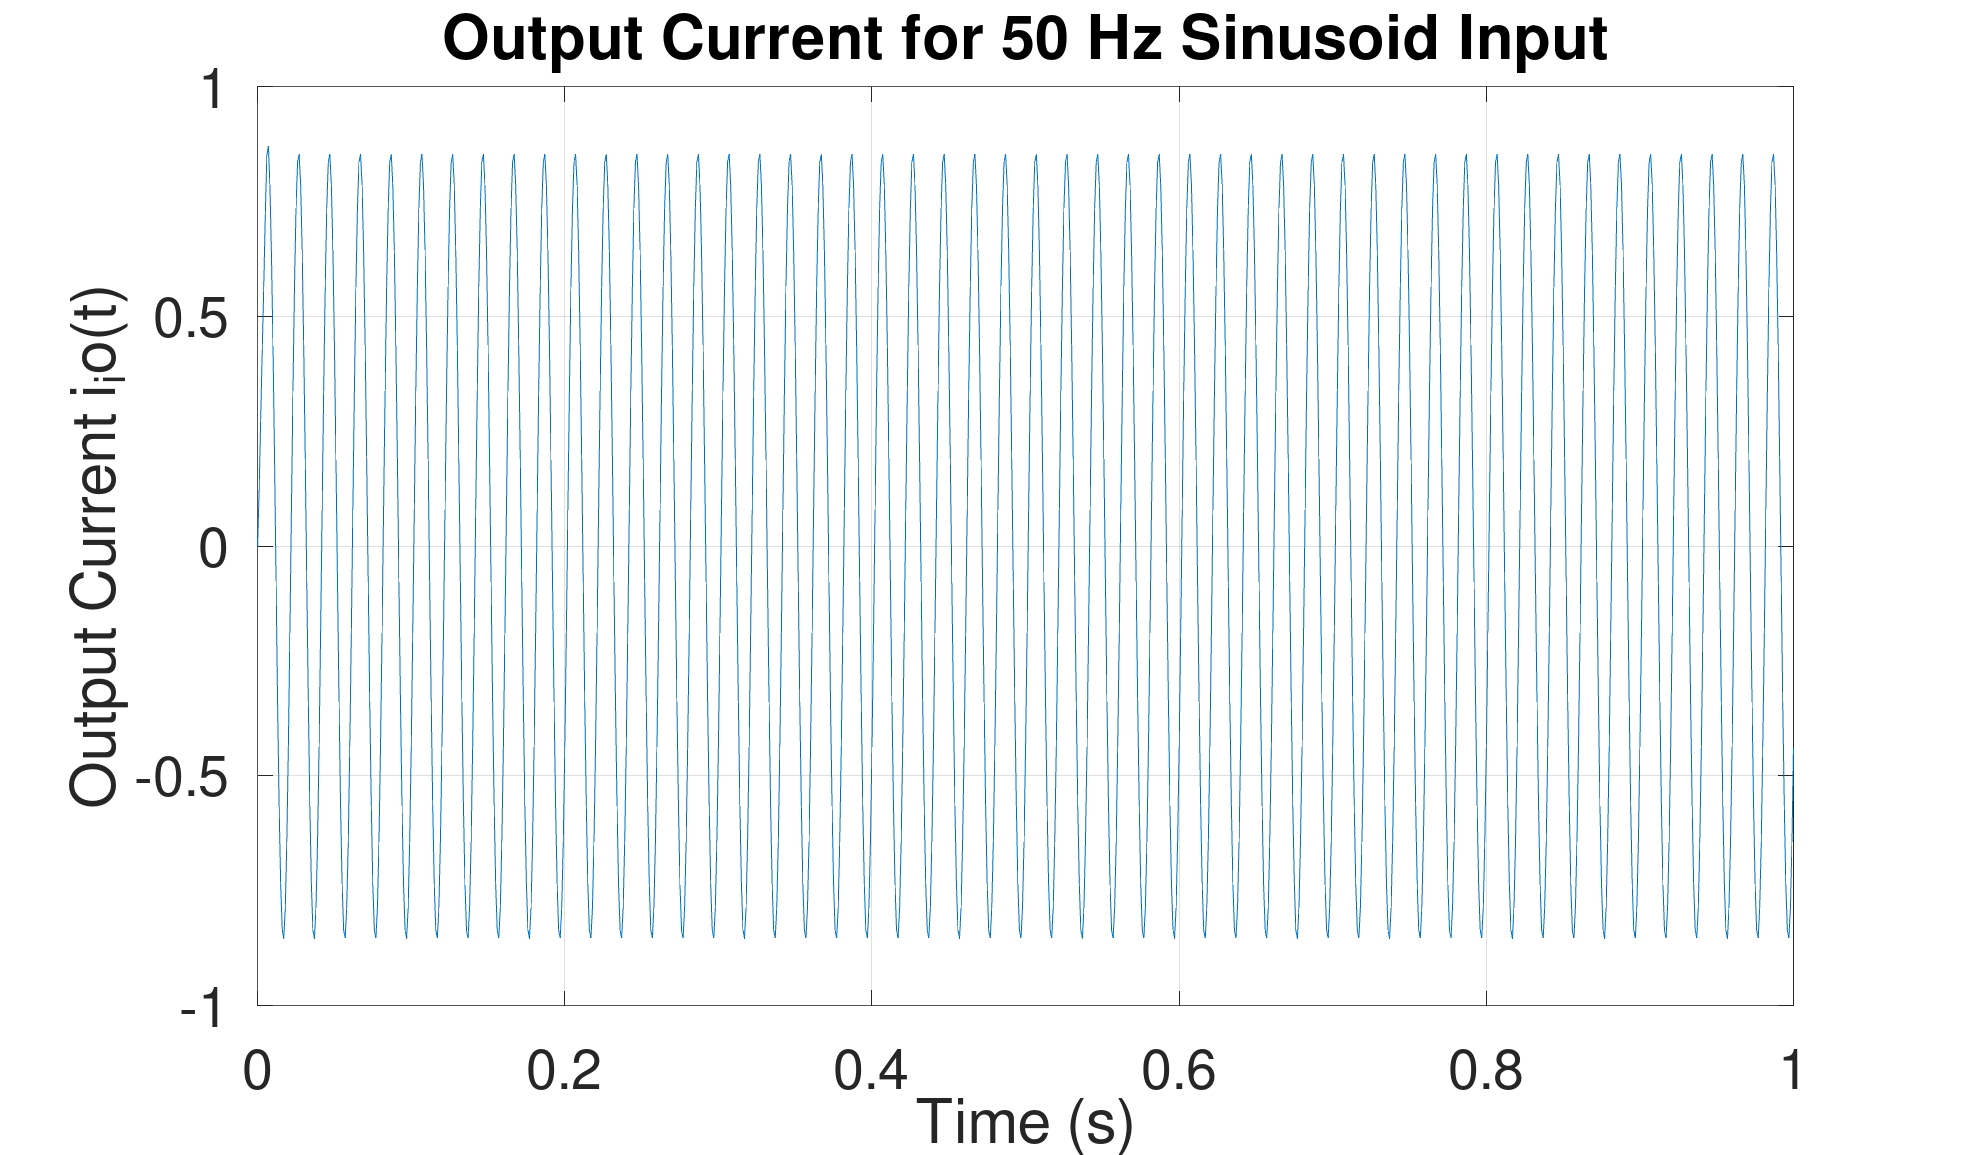
\includegraphics[width=.9\linewidth]{ENG204-Assignment-4-50Hz.png}
\caption{Response of the system when 50Hz sine wave is applied.}
\end{figure}
\end{FIGURE}
\begin{FIGURE}
\begin{figure}[H]
\centering
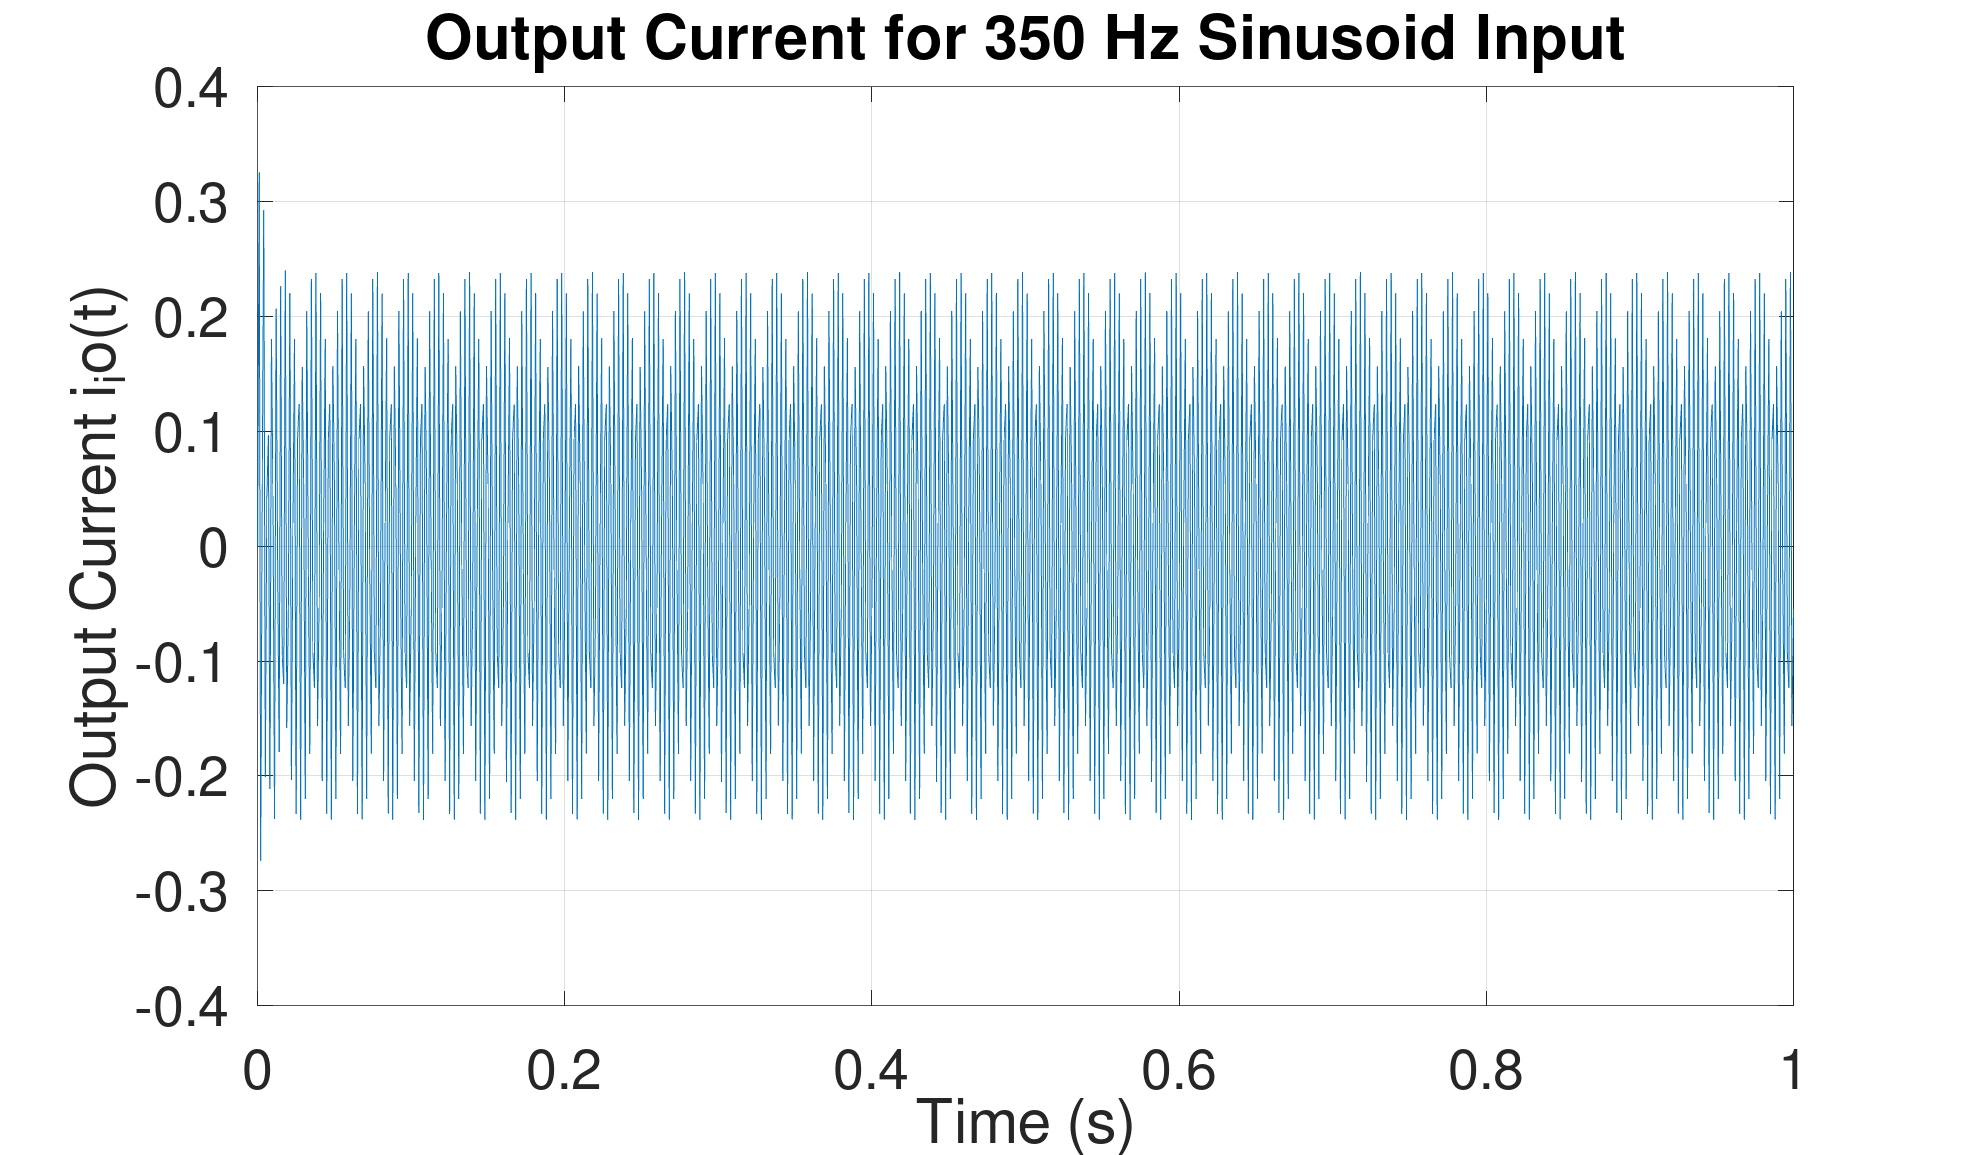
\includegraphics[width=.9\linewidth]{ENG204-Assignment-4-350Hz.png}
\caption{Response of the system when 350Hz sine wave is applied.}
\end{figure}
\end{FIGURE}
\begin{FIGURE}
\begin{figure}[H]
\centering
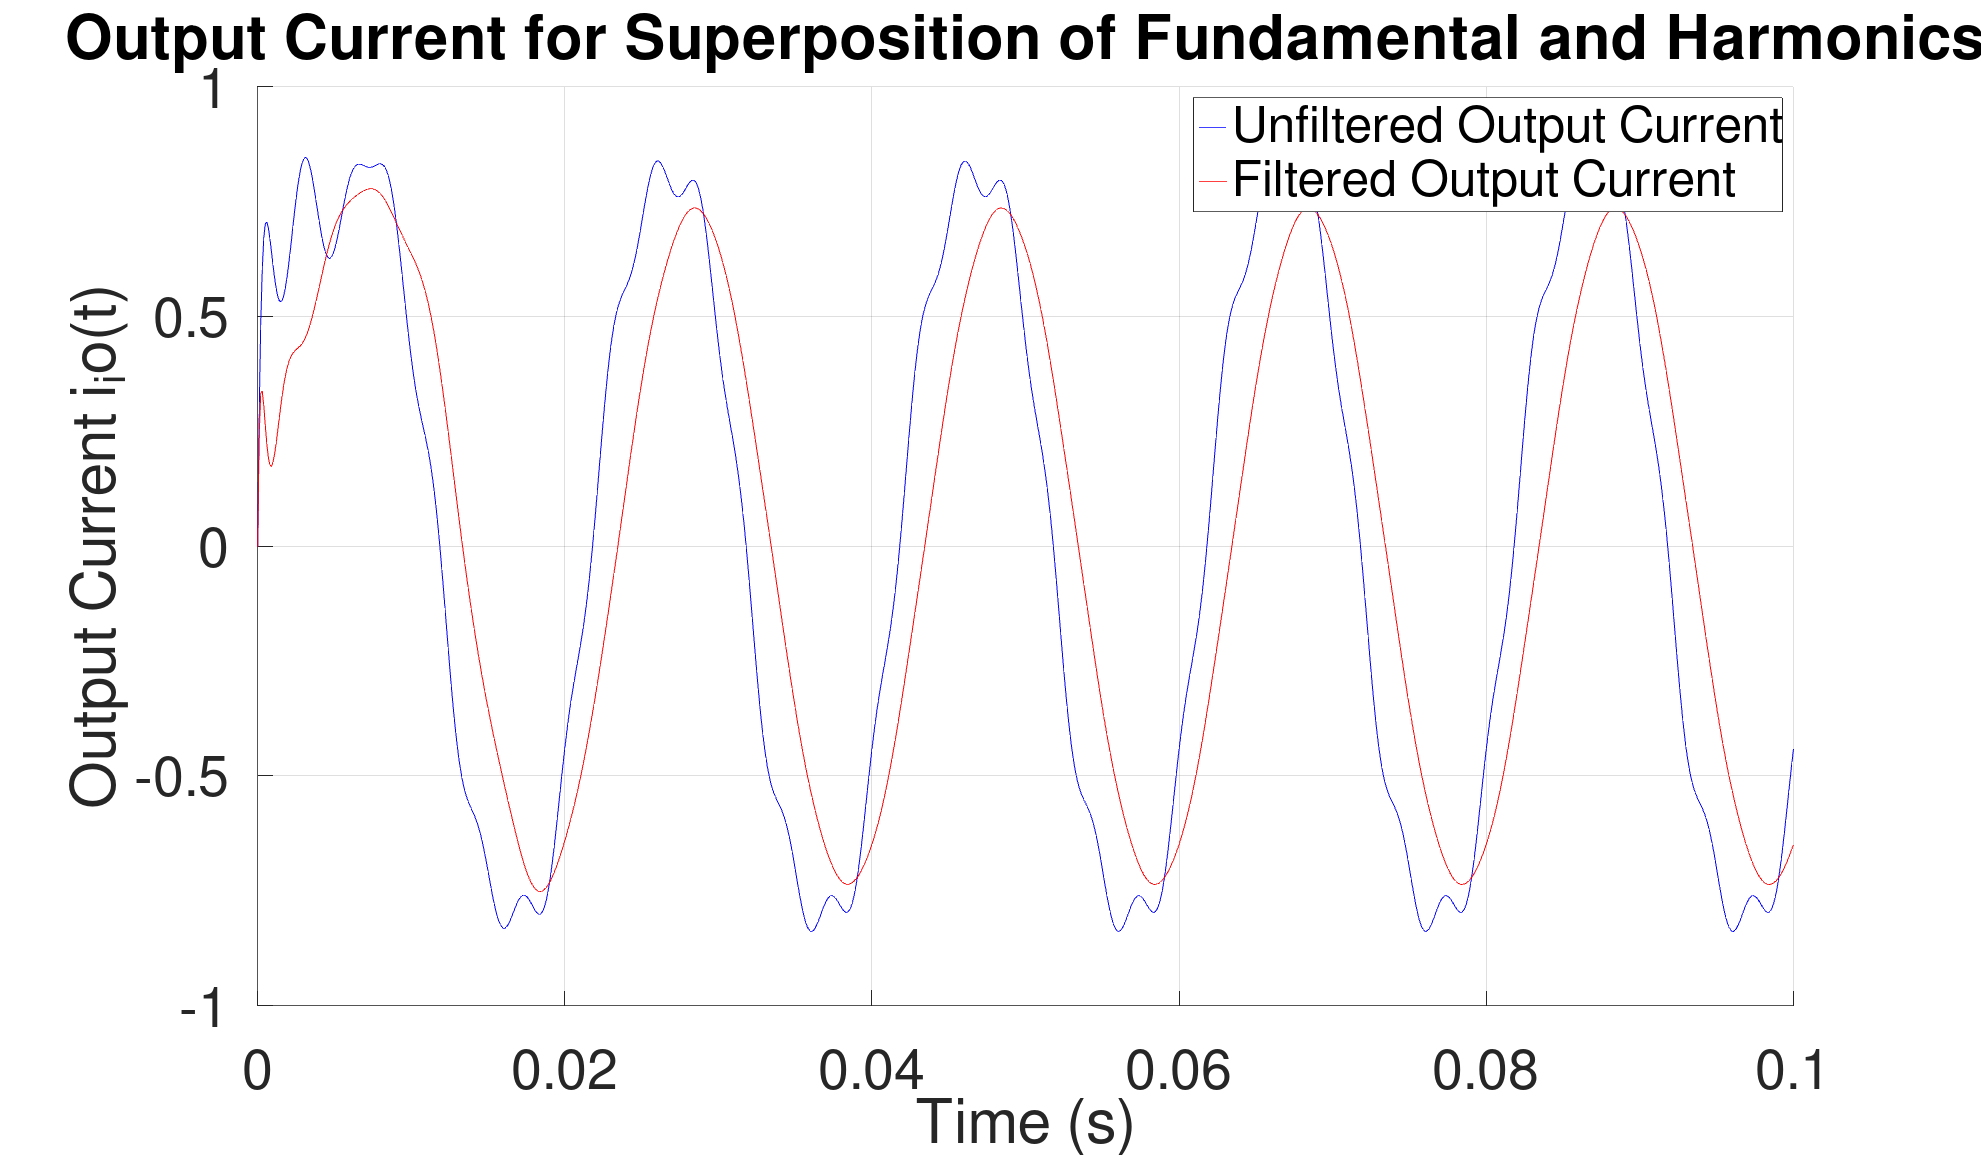
\includegraphics[width=.9\linewidth]{ENG204-Assignment-4-Super.png}
\caption{Response of the system when a sum of the harmonic frequencies is applied.}
\end{figure}
\end{FIGURE}
\subsection{Impulse Response}
\label{sec:orga0a5b7c}
The oscillations in the impulse response suggest a damped system because the oscillations gradually decay. The way in which the signal decays suggest an underdamped system because of the overshoot. The high initial amplitude change indicates a fast transient response, indicating a high-quality factor or resonance. This could lead to instability if the damping is not sufficient. These characteristics may not be ideal for power systems due to the large amplitude reaction sudden disturbances.
\subsection{State Space Representation}
\label{sec:org98180e3}
The general form of:
\[q[n + 1] = Aq[n] + Bx[n]\]
\[y[n] = Cq[n] + dx[t]\]
Where:
\begin{itemize}
\item Matrix A: Describes the internal dynamics of the system.
\item Matrix B: Describes how the input affects the system.
\item Matrix C: Maps the state to the output.
\item Matrix D: Represents direct feedthrough from input to output.
\item Matrix A is helpful to determine the stability of the system through its eigenvalues.
\end{itemize}
Matrix B,C and D describe how the system can be controlled and monitored, an important property for power systems.
\subsection{System Response and Its Utility in Power Systems}
\label{sec:org8ec8367}
The Bode plot shows significant attenuation of the n1 and n2 harmonics, which implies successful blocking of these frequencies. This helps the power system to remain stable through harmonic current injections. The filtering stabilises the effective power transfer and system efficiency.
The step response of the system shows that after a transient the system will settle to a steady state. This is useful in power systems to ensure reliability when there are fluctuating loads or transient conditions
\end{document}
